% Candidate; source page 405. Dashed edges meet at hidden C.
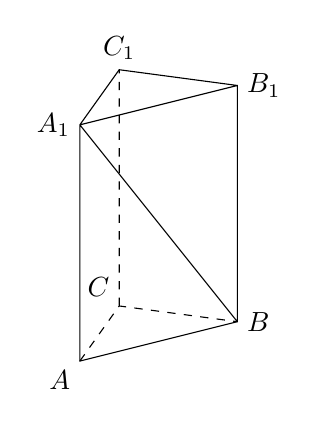
\begin{tikzpicture}[scale=1,>=stealth]
\coordinate (A) at (0,0); \coordinate (B) at (2,.5); \coordinate (C) at (.5,.7);
\coordinate (A1) at (0,3); \coordinate (B1) at (2,3.5); \coordinate (C1) at (.5,3.7);
\draw (A)--(B)--(B1)--(A1)--cycle (A1)--(C1)--(B1) (A1)--(B);
\draw[dashed] (A)--(C)--(B) (C)--(C1);
\node[below left] at (A) {$A$}; \node[right] at (B) {$B$}; \node[above left] at (C) {$C$};
\node[left] at (A1) {$A_1$}; \node[right] at (B1) {$B_1$}; \node[above] at (C1) {$C_1$};
\end{tikzpicture}
